% 0510(본책 92쪽) — P 에서 두 직선 PAB·PDC, AC·BD·BC, ∠P=40°, ∠PAC=105°, ∠ABD=x(색칠). 다시 그림.
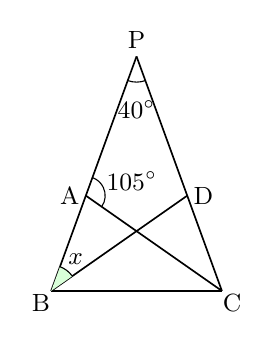
\begin{tikzpicture}[scale=1.02, line width=0.6pt]
  \draw (-0.000,2.635) -- (-1.063,-0.285);
  \draw (-0.000,2.635) -- (1.063,-0.285);
  \draw (-0.631,0.901) -- (1.063,-0.285);
  \draw (-1.063,-0.285) -- (0.631,0.901);
  \draw (-1.063,-0.285) -- (1.063,-0.285);
  \draw[line width=0.4pt] (-0.109,2.334) arc[start angle=-110.000, end angle=-70.000, radius=0.320];
  \node[font=\small, inner sep=0.5pt] at (-0.000,1.975) {$40^\circ$};
  \draw[line width=0.4pt] (-0.434,0.763) arc[start angle=-35.000, end angle=70.000, radius=0.240];
  \node[font=\small, inner sep=0.5pt] at (-0.059,1.081) {$105^\circ$};
  \fill[green!15] (-1.063,-0.285) -- (-0.800,-0.101) arc[start angle=35.000, end angle=70.000, radius=0.320] -- cycle;
  \draw[line width=0.4pt] (-0.800,-0.101) arc[start angle=35.000, end angle=70.000, radius=0.320];
  \node[font=\small, inner sep=0.5pt] at (-0.758,0.112) {$x$};
  \node[font=\small, inner sep=1.5pt] at (-0.000,2.835) {P};
  \node[font=\small, inner sep=1.5pt] at (-0.831,0.901) {A};
  \node[font=\small, inner sep=1.5pt] at (0.831,0.901) {D};
  \node[font=\small, inner sep=1.5pt] at (-1.191,-0.438) {B};
  \node[font=\small, inner sep=1.5pt] at (1.191,-0.438) {C};
\end{tikzpicture}
